\documentclass[dvipdfmx,titlepage,a4j]{jsarticle}

\usepackage{url}
\usepackage{graphicx}
\usepackage{listings,jvlisting}
\usepackage{amsmath,amssymb}
\usepackage{graphicx}
\usepackage[yen]{okuverb}
\usepackage{ascmac}
\usepackage{fancybox}
\usepackage{fancyvrb}
\usepackage{fancyhdr}
\usepackage{lastpage}
\usepackage{caption}
\usepackage{subcaption}
\usepackage{here}

\fancypagestyle{foot}
{
\fancyhead[C]{}
\fancyfoot[C]{\thepage / \pageref{LastPage}}
\renewcommand\headrulewidth{0.4pt}
}

%ここからソースコードの表示に関する設定
\lstset{
  language={C++},
  basicstyle={\ttfamily},
  identifierstyle={\small},
  commentstyle={\smallitshape},
  keywordstyle={\small\bfseries},
  ndkeywordstyle={\small},
  stringstyle={\small\ttfamily},
  frame={tb},
  tabsize={2},
  breaklines=true,
  columns=[l]{fullflexible},
  numbers=left,
  xrightmargin=0zw,
  xleftmargin=3zw,
  numberstyle={\scriptsize},
  stepnumber=1,
  numbersep=1zw,
  lineskip=-0.5ex
}

\title{タイトル}
\author{waarrk}
\date{2023年2月1日}

\begin{document}

\begin{titlepage}
    \centering
    \vspace*{2cm}

    \vspace{1cm}

    {\LARGE \textbf{DPマッチングによる単語音声認識}}

    \vspace{0.5cm}

    {\LARGE 2024年度開講 認識工学レポート}

    \vspace{1.5cm}

    {\textbf{千葉工業大学 先進工学部 未来ロボティクス学科}\\}
    {\textbf{22C1704 鷲尾 優作}}

    \vfill

    {\large 2024年6月19日}

    \vspace{1cm}
\end{titlepage}

\section{目的}
本稿では,DPマッチングを用いた単語音声認識の手法について実験を行い,その正答率を評価することで,単語音声認識におけるDPマッチングの有効性を検証する.

\section{実験}
実験には,単語音声認識のための音声データセットを用いる.
音声入力から音声分析までの過程は既に終了しているものとし,あらかじめ用意された音声データセットを用いて,DPマッチングによる単語音声認識を行う.

\subsection{DPマッチング}
DPマッチングは,動的計画法を用いて,2つの系列データ間の類似度を計算する手法である.
2つの系列データを比較し,最も類似度の高い経路を探索することで,系列データ間の類似度を計算する.
類似度は,探索した経路の経路長が短いほど高くなる.
本実験では,音声データのメルケプストラム特徴量を用いて,DPマッチングによる単語音声認識を行う.

\subsection{データの内容}
音声データセットは,2名が2回ずつ発声した100単語のデータで構成されている.
内容は,100単語の地名単語データベースであり,各単語は日本国内の地名を表すものである.
話者2名がそれぞれ2回ずつ発声した計400単語のメルケプストラム特徴量が記録されており,
話者1の1回目「city011」話者1の2回目「city012」話者2の1回目「city021」話者2の2回目「city022」の4つのデータが含まれている.

\subsection{実験手順}
本実験では,1音声データに対し,もうひとつの100単語を順番に比較し,DPマッチングにより最も類似度の高い単語を認識する.
また,比較は同一話者による音声データ同士,別話者による音声データ同士の2通りで行い,計6通りの組み合わせで正答率を比較する.

比較にはListing \ref{code:main.py}に示すPythonスクリプトを用いた.

\subsection{実験結果}
実験結果を表\ref{table:result}に示す.
表中の「同一話者」は,同一話者による音声データ同士の比較結果を示し,「別話者」は別話者による音声データ同士の比較結果を示す.
同一の比較にあたる部分は空欄としている.

\begin{table}[H]
    \begin{center}
        \caption{DPマッチングによる単語音声認識の正答率}
        \begin{tabular}{c|c|c|c} \hline
            比較した話者   & 話者1(1回目) & 話者1(2回目) & 話者2(1回目) \\ \hline
            同一話者     & 99\%     &          & 99\%     \\
            別話者(1回目) & 90\%     & 92\%                \\
            別話者(2回目) & 84\%     & 86\%                \\ \hline
        \end{tabular}
        \label{table:result}
    \end{center}
\end{table}

\section{考察}
表\ref{table:result}より,同一話者による音声データ同士の比較では,2つのデータでそれぞれ99\%と最も高い正答率を示した.
一方,別話者による音声データ同士の比較では,正答率が10\%程度低下している.
これは,同一話者による音声データ同士の方が,発声の特徴が類似しているため,DPマッチングによる認識が容易であること,
別話者の場合,発声の特徴が異なるため,DPマッチングによる認識が難しくなることを示すと考えられる.

検証のため,DPマッチングにより得られた経路をバックトラックし,認識結果を確認した.
図 \ref{fig:dp_matching_011_012}に,話者1の1回目「city011」と話者1の2回目「city012」の音声データを比較した結果,
図 \ref{fig:dp_matching_011_021}に,話者1の1回目「city011」と話者2の1回目「city021」の音声データを比較した結果を示す.

それぞれ,図中の赤い線がDPマッチングにより得られた経路を表し,100単語の最も最初のデータである「AZABU」を認識した結果を示している.

\begin{figure}[htbp]
    \centering
    \begin{minipage}[b]{0.45\linewidth}
        \centering
        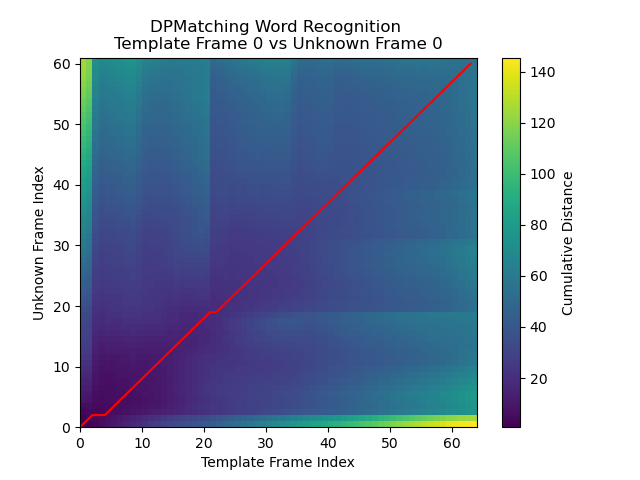
\includegraphics[width=\linewidth]{picture/city011_000_vs_city012_000.png}
        \caption{話者1の1回目「city011」と話者1の2回目「city012」の音声データを比較した結果}
        \label{fig:dp_matching_011_012}
    \end{minipage}
    \hspace{0.05\linewidth}
    \begin{minipage}[b]{0.45\linewidth}
        \centering
        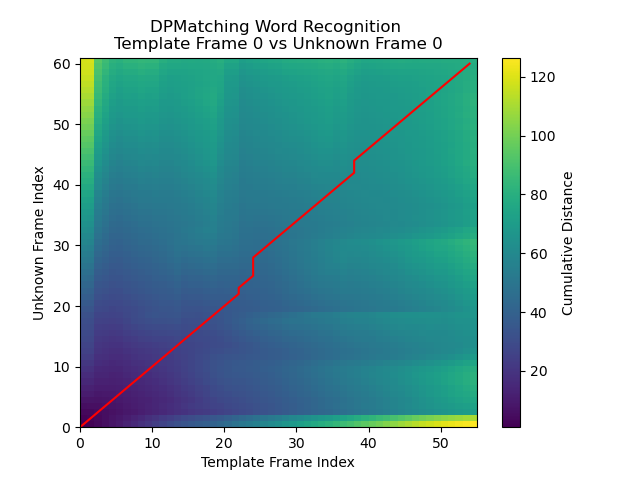
\includegraphics[width=\linewidth]{picture/city011_000_vs_city021_000.png}
        \caption{話者1の1回目「city011」と話者2の1回目「city021」の音声データを比較した結果}
        \label{fig:dp_matching_011_021}
    \end{minipage}
\end{figure}

両画像とも,赤い線が左上から右下に向かって伸びていることから,DPマッチングにより正しく認識されたことが確認できる.
この経路の距離が短いほど,認識精度が高くなるが,図\ref{fig:dp_matching_011_021}はほぼ直線の図\ref{fig:dp_matching_011_012}に比べて
ギザギザした経路となっていることから,認識精度が低いことが示されている.

このことは,表\ref{table:result}の結果と一致しており,別話者による音声データ同士の比較では,正答率が低下することが確認された.


\section{結論}
本稿では,DPマッチングを用いた単語音声認識の手法について実験を行い,その正答率を評価した.
実験結果より,同一話者による音声データ同士の比較では,DPマッチングによる認識が容易であることが示された.
一方,別話者による音声データ同士の比較では,正答率が低下することが確認された.

\newpage

\lstinputlisting[caption=main.py,label=code:main.py,firstline=1,lastline=153,firstnumber=1,]
{../main.py}

\nocite{*}
\bibliographystyle{jplain}
\bibliography{refs}

\end{document}
